%----------------------------------------------------------------------------------------
%	PACKAGES AND OTHER DOCUMENT CONFIGURATIONS
%----------------------------------------------------------------------------------------

\documentclass[14pt]{SelfArx} % Document font size and equations flushed left
\usepackage[english]{babel} % Specify a different language here - english by default
\usepackage{amsmath}
%\usepackage{textgreek}
\usepackage{caption}
\usepackage{eqnarray}
\usepackage{hyperref}
\usepackage[T1]{fontenc} % Ligaturen, richtige Umlaute im PDF
\usepackage[utf8]{inputenc}% UTF8-Kodierung für Umlaute usw
\DeclareGraphicsExtensions{.pdf,.png,.jpg,.tif} % bevorzuge pdf-Dateien
\usepackage[]{natbib}
%\usepackage{placeins}
\usepackage{lipsum}
\numberwithin{equation}{section}

\usepackage{subscript}
\usepackage{lipsum} % Required to insert dummy text. To be removed otherwise

%----------------------------------------------------------------------------------------
%	COLUMNS
%----------------------------------------------------------------------------------------

\setlength{\columnsep}{0.55cm} % Distance between the two columns of text
\setlength{\fboxrule}{0.75pt} % Width of the border around the abstract

%----------------------------------------------------------------------------------------
%	COLORS
%----------------------------------------------------------------------------------------

\definecolor{color1}{RGB}{0,0,90} % Color of the article title and sections
\definecolor{color2}{RGB}{0,20,20} % Color of the boxes behind the abstract and headings

%----------------------------------------------------------------------------------------
%	HYPERLINKS
%----------------------------------------------------------------------------------------

\usepackage{hyperref} % Required for hyperlinks
\hypersetup{hidelinks,colorlinks,breaklinks=true,urlcolor=color2,citecolor=color1,linkcolor=color1,bookmarksopen=false,pdftitle={Title},pdfauthor={Author}}

%----------------------------------------------------------------------------------------
%	ARTICLE INFORMATION
%----------------------------------------------------------------------------------------

\JournalInfo{C12 - Theory of Neural Dynamics} % Journal information
\Archive{Protocol}

\PaperTitle{Differences between Gaussian and randomly connected neurons for light-stimulated neural networks } % Article title

\Authors{Norman Seeliger\textsuperscript{1}, Jannik Luboeinski\textsuperscript{2}*, Dr. Tatjana Tchumatchenko\textsuperscript{3}} % Authors
\affiliation{\textsuperscript{1}\textit{Module C12 of the master program “Interdisciplinary Neuroscience”}} 
\affiliation{\textsuperscript{2}\textit{Masters student, Group for Theory of Neural Dynamics, Max Planck Institute for Brain Research, Frankfurt, Germany. }}
\affiliation{\textsuperscript{3}\textit{Director and Group Leader, Group for Theory of Neural Dynamics, Max Planck Institute for Brain Research, Frankfurt, Germany. }}
\affiliation{*\textbf{Supervision}} % Corresponding author
\Keywords{Gaussian connections - Optogenetics - neural network} 
\newcommand{\keywordname}{Keywords} 

%----------------------------------------------------------------------------------------
%	ABSTRACT
%----------------------------------------------------------------------------------------

\Abstract{
Artificial neural networks are of high significance for computational and theoretical neuroscience since they allow predictions about the collective behavior of a group of neurons to various stimuli. Especially when being combined with optogenetics, which by itself offers fine-grained and specifically targeted stimulations of genetically modified and thus light-sensitive neurons, the boundaries of natural recordings not being feasible for large groups of neurons can be surpassed to shed light on new insights of the ensemble.\newline
It has recently been shown that by the usage of a 3-state Markov model of Channelrhodopsin-2 together with a Leaky Integrate-and-Fire neuron model, networks of randomly connected artificial neurons can be implemented and tested to obtain quantitative predictions of the oscillating response under a light  stimulus. This approach is here extended by applying Gaussian distributed connectivity patterns for all connections drawn between individual neurons.

The results of the thus created network showed a stronger representation of the stimulus within the network allowing for higher peaks and well-defined depths of firing rates for the excitatory and inhibitory population. The spatial firing rate distribution of the latter additionally showed, in strong contrast to the random connection pattern, a very high resemblance to the applied stimulus by capturing its main characteristics. \newline
}

%----------------------------------------------------------------------------------------

\begin{document}
\flushbottom % Makes all text pages the same height
\maketitle % Print the title and abstract box
\tableofcontents % Print the contents section
\thispagestyle{empty} % Removes page numbering from the first page


%----------------------------------------------------------------------------------------
%	ARTICLE CONTENTS
%----------------------------------------------------------------------------------------
\renewcommand{\baselinestretch}{1.2}\large
%\fontsize{14}{12}
\section{Introduction} 
When trying to understand neural behavior under specific circumstances, the usage of artificial neural networks has been proven to be of big avail for various situations. \newline
In general, artificial neural networks are constructed similarly to biological neural networks by assigning tasks to be performed simultaneously by the whole population, which makes them a very powerful tool for statistics, cognitive psychology and artificial intelligence, as well as a versatile cornerstone of theoretical and computational neuroscience. \newline
Within the mentioned field of computational neuroscience, each individual neuron is constructed following a mathematical description of a real cell's properties to achieve biologically realistic, yet reduced models aiming to capture the characteristic behaviors of different neuron types. \newline These models can be distinguished into pharmacological input neuron models following natural stimulation and delivering the probability of a spike due to this input as well as membrane voltage models, which produce predictions of the cell membrane's voltage change due to electrical stimulation of the neuron. While the first subdivision incorporates models as the two state Markov model of \cite{Nossenson} and the non-homogeneous Poisson process model by \cite{siebert}, the latter comprises not only one of the most commonly known and heavily used models of a neuron as implemented by \cite{Hodgkin}, but also allows for various ways of sub-cellular and detailed integration by the usage of (Leaky) Integrate-and-Fire neuron models (\cite{abbott}).\newline
\newline
For the simultaneous activity of the whole network allowing synchronized and oscillating behavior and being determinative over the negligible single-neuron dynamics, those Leaky Integrate-and-Fire neuron models are an appropriate choice and used here to implement a population of neurons within an neural network to perform an optogenetic analysis. \newline
Optogenetics has an advantage over normal stimulations within the brain via electrical currents for it can very precisely target specific neurons and therefore lead to more traceable and reproducible results. On this account and since its earliest approaches by \cite{zemelman}, many studies and profound findings have been made possible due to optogenetic facilitation including for example the contribution of the amygdala to fear conditioning by \cite{Haubensak}, the treatment of Parkinson (\cite{gradinaru}) or the restoration of auditory activity in dead mice (\cite{hermandez}). \newline
All of these experiments share the underlying principle of optogenetic stimulation by rendering the neurons sensitive to a light stimulus. This is done by genetically modifying specific cells to express light sensitive proteins as channelrhodopsin or halorhodo-psin of which the recording can be performed in a spatiotemporal well defined manner by applying light to those neurons and measure e.g. the vesicular and neurotransmitter release or the change in membrane potential. While this is feasible for smaller groups or single neurons, the investigation of large networks is difficult due to the time scales of rhodopsins and neurons and further hindered by the problem of simultaneous recordings of large groups of neurons. For artificial neural networks within the topic of theoretical neuroscience however, Channelrhodopsin-2 can be modeled using a 3-state Markov model and, by varying the frequency and intensity of induced light pulses, detailed activities of a network under different circumstances can be investigated to achieve quantitative predictions of the network's behavior under optogenetic stimulation (\cite{jannik}).\newline
\begin{figure} [h]
\centering
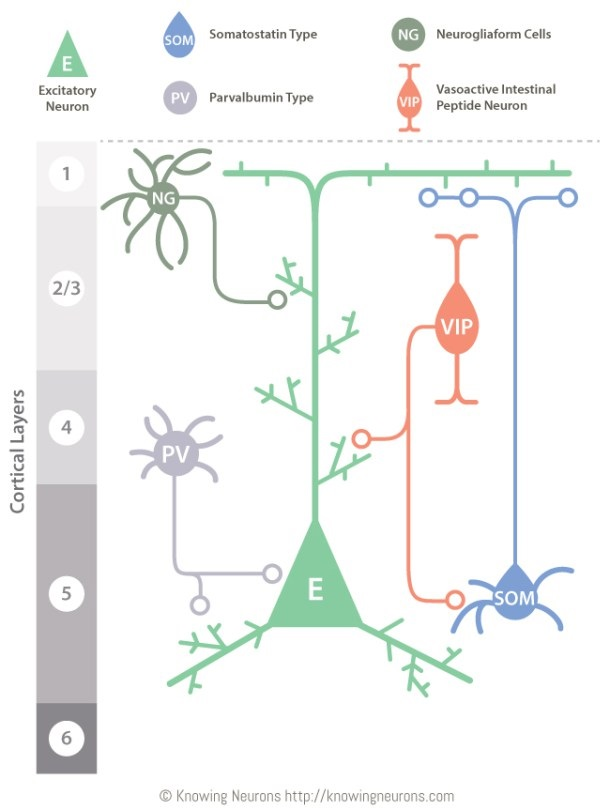
\includegraphics[width = 0.5\textwidth]{brainnetwork.png}
\caption{\textbf{Exemplar neural circuit.}}
\label{fig:brainnetwork}
\end{figure}
\newline
What is additionally important for the reaction of a network to an applied stimulus, are not only the parameters of the input into a single neuron but also the connectivity of the network. In cortical, cerebellar and hippocampal brain regions, local neural circuits are not only comprised of excitatory neurons (mostly pyramidal neurons) but incorporate different kinds of inhibitory neurons shaping and influencing the corresponding response to a stimulus (see Figure \ref{fig:brainnetwork}). This leads for example to the shaping of orientation and direction tuning within the visual cortex (\cite{Crook}) or to oscillating behavior of natural brain networks (\cite{salinas}, \cite{engel}).\newline
Of those inhibitory interneuons, the two main types are the parvalbumin (PV) and somatostatin (SOM) making up 40 \% and 25 \% of the total inhibitory subpopulation, respectively. Being either Basket cell like (PV, hippocampus and cortex layers 2-6) or Martinotti cell like (SOM, e.g. cortex layers 2-6), those neurons tend to connect to neighboring neurons based on their distance to them, forming smaller local groups delivering input to those inhibitory neurons. This can be seen on a macroscopic level as well, taking into account small world networks of the brain and the tendency of neurons to dense clustering (\cite{Bassett}) by drawing only few longer connections to different clusters.\newline
\newline
In this module, the goal was thus defined as to use an artificial neural network with light-sensitive channels implemented within Leaky Integrate-and-Fire neuron models and to extend the there used random connectivity pattern to Gaussian distributed connectivity patterns within the excitatory and inhibitory population, therefore considering the tendency of neurons to connect to close neurons rather than neurons further away. The resulting network is then analyzed using the same techniques as in the original version to enable comparisons of the network under different connectivity topologies for varying light stimuli.
\section{Material and Methods}
For the analysis performed in this module, the neural network implemented by \cite{jannik} has been used. \newline
The aspects of special importance for the results obtained here as well as the basics behind the model are described below. \newline
For the way of computation of firing rates see the work cited above.
\subsection{Leaky Integrate-and-Fire model}
The whole network consists of 4500 neurons, of which 3600 are excitatory and 900 inhibitory, being partially connected to each other either in a random pattern or by considering a Gaussian distribution (see Chapter \ref{sec:network}).\newline
For each neuron of the network, the Leaky Integrate-and-Fire neuron model (following LIF) has been used to simulate voltage dynamics and spike generation, including a leakage term V modeling the membrane conductance. \newline 
\newline
In the LIF model, input currents arriving at the neuron are summed up and, given that a specific threshold criterion $V_{th}$ has been reached, generate an implicit action potential. After this action potential, which delivers no information about its shape but is rather a formal event described by a firing time $t^{f}$, the membrane potential is set to a specific reset value $V_{reset}$. \newline
Every neuron hereby is considered to consist of a capacitor \textit{C} in parallel with a resistor \textit{R} which are driven by a input current according to Equation \ref{eq:lifgen1}. Here, the resistive current $I_{R}$ passes through the resistor and can be calculated following Ohm's law as $I_{R} = u(t)/R$ whereas the capacitive current charges the capacitor \textit{C} and can be subbed as $C = q/u$ or, with respect to time, as $q = C * \frac{du}{dt}$ (with q being the charge).
\begin{equation}
\label{eq:lifgen1}
I_{synapse}(t) = I_{R}(t) + I_{C}(t)
\end{equation}
By introducing the membrane time constant $\tau_{m} = R*C$, multiplying the equation with R and using the conductance instead of the membrane resistance (which is only the inverse, $g = 1/R$), one obtains the standard form for LIF model neurons as is shown in Equation \ref{eq:lifgen2}. \newline
\begin{equation}
\label{eq:lifgen2}
\tau_{m} \frac{du}{dt} = -u(t) + R* I_{synapse}(t)
\end{equation}
\newline
Additionally to the synaptic input current into the LIF neuron model, there is a factor originating from an external light stimulus onto the network and individual neurons. Thus, the total input current for a singe neuron has to be computed as given in Equation \ref{eq:lifgen3} to not only consider the dynamics of synaptic input current, but to additionally account for the contribution of Channelrhodopsin-2 channels which is explained along with the influencing stimulus in more detail in Chapter \ref{sec:stimulus}. \newline
\begin{equation}
\label{eq:lifgen3}
\tau _{m} \frac{du}{dt} = -u(t) + R* ( I_{synapse}(t) + I_{Chr2}(t,u))
\end{equation}
Furthermore, the synaptic input current itself consists of not only general input from distal neurons (modeled as Brownian motion through an Ornstein-Uhlenbeck process and driven by Gaussian white noise) but of internal currents originating from other neurons which are nearby and explicitly modeled within the network. This additive input current coming from the network a single neuron belongs to is further explained in Chapter \ref{sec:network}.  \newline
\subsection{Light sensitivity and stimulus}
\label{sec:stimulus}
Each neuron incorporates light-sensitive \newline Channelrhodopsin-2 channels whose dynamics are described using a 3-state model originally proposed by \cite{nagel}. \newline
Here, the channels switch between an Open, Closed and Desensitized state with different transition probabilities and possible influence of a light stimulus. The effective conductance of a channel population depends on the number of channels (of which there are two different values used: 60000 and 300000), the probability of such a channel being open and its conductance given the open state.\newline
Light stimuli were applied to single neurons via pulses of 4 ms duration and a frequency of 50 Hz. In the network, the stimulus light intensity was spatially Gaussian-distributed with its center in the middle of the network.
\newline
For the stimulation of the network as a whole, the individual light intensity arriving at a neuron in row \textit{n} and column \textit{m} (for the general structure of the network, please see \ref{sec:network}) can be expressed as in Equation \ref{eq:lightstim} (with $n_{c}$ and $m_{c}$ being the center of the population and $\sigma_{light}^{2}$ being the variance of the spatial Gaussian distribution of the light stimulus) and is depicted in Figure \ref{fig:irradiancemap}. \newline
\begin{equation}
\label{eq:lightstim}
E(n,m) = \dot{E}*exp(- \frac{(n-n_{c})^{2}+(m-m_{c})^{2}}{2*\sigma_{light}^{2}})
\end{equation}
\begin{figure} [htp]
\centering
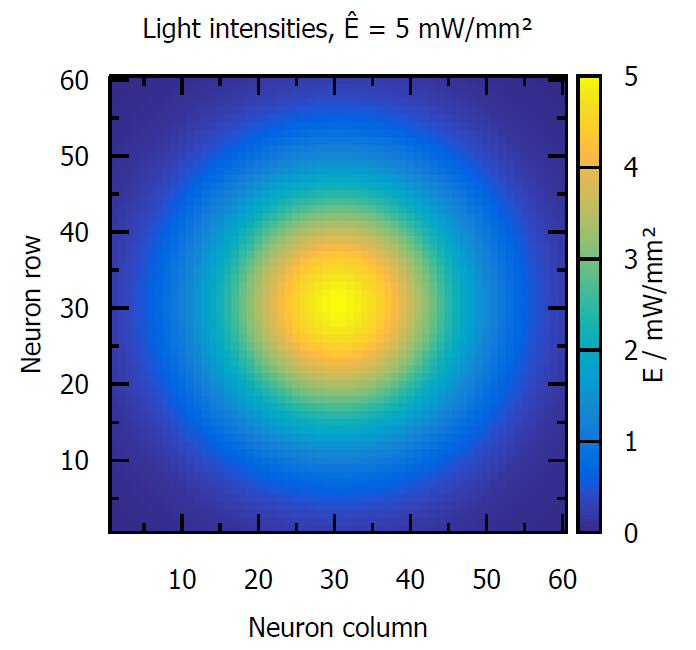
\includegraphics[width = 0.45\textwidth]{irradiancemap.png}
\caption{\textbf{Irradiance map for network.} Shown are the light stimuli as applied to the whole excitatory population of \textit{N = 3600} neurons in  spatial Gaussian distribution.}
\label{fig:irradiancemap}
\end{figure}
\subsection{Connectivity patterns}
\label{sec:network}
Every neuron is embedded in the network and thus receives input from other neurons as well as delivers output, which is true for both inhibitory and excitatory neurons in different ways and depending on the coupling strength as well as on the connection patterns. \newline
To maintain the ratio of 4 to 1 between excitatory and inhibitory neurons within a uniform spatial ordering, a specific pattern for the network has been chosen (see Figure \ref{fig:connschema}). Every neuron is given its location within the network (being a 120 times  120 matrix) and a connection between two separate neurons is established when a specific criterion depending on the general pattern is met. 
\begin{figure} [htp]
\centering
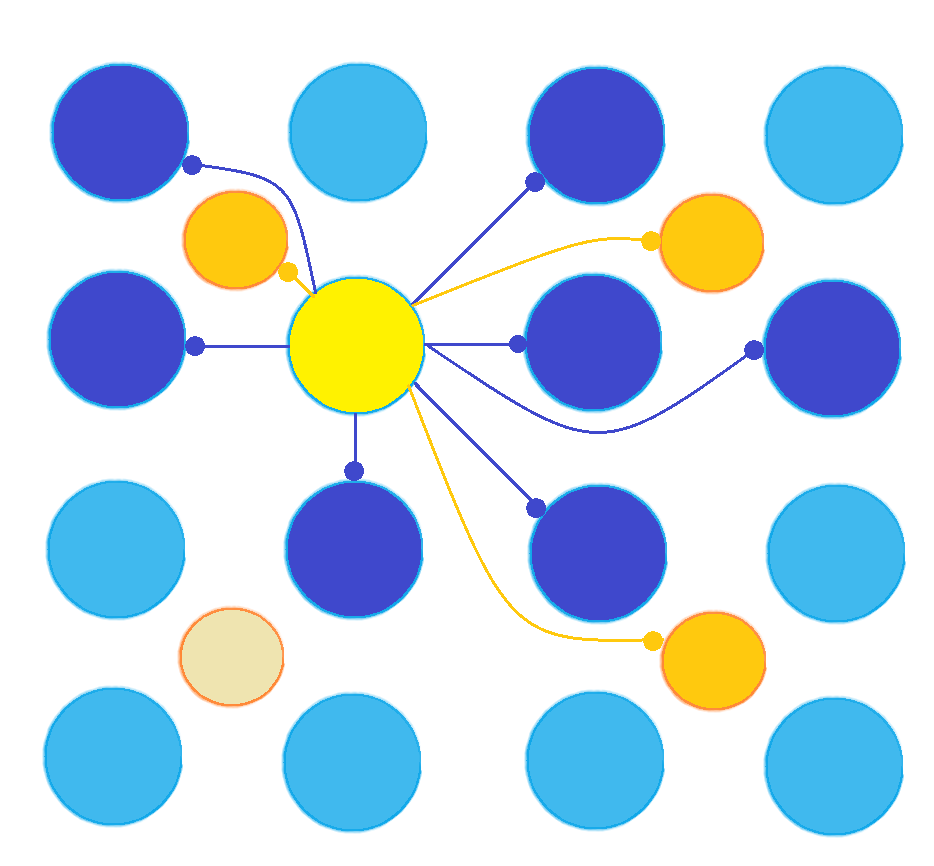
\includegraphics[width = 0.45\textwidth]{connschema.png}
\caption{\textbf{Schematic connectivity pattern and spatial ordering.} For every four excitatory neurons, there is one inhibitory neuron in the center. This pattern is repeated over the network. Shown are exemplary connections of a specific neuron (yellow) to other excitatory (blue and deep blue) and inhibitory neurons (ocher).}
\label{fig:connschema}
\end{figure}
\newline
For the completely random connection pattern, values are drawn out of a uniformly random distribution and, given that this value falls below the connection probability \textit{PC}, a synapse is formed. \newline
For the Gaussian connectivity pattern, the connection probability was replaced with a value originating from a Gaussian distribution as is shown in Equation \ref{eq:gauss} with $\sigma^{2}$ and \textit{amp} being the variance and amplitude of the distribution and distance the distance between two neurons. Thus, neurons being farther apart have a smaller chance to be connected than neurons which are close to each other. The individual values for amplitude and deviation differ depending on the neuron type and amount of connections which had to be established. A summary is given in Table \ref{tab:ampsigs}, an exemplar connection map is depicted in Figure \ref{fig:connmap}. The values for the Gaussian distributions have been chosen only with a qualitative instead of a quantitative character and are therefore arbitrary.
\newline
\begin{equation}
\label{eq:gauss}
random < amp * \exp^{-\frac{distance}{2*\sigma^{2}}}
\end{equation}
\begin{table}[htb]
\centering
\caption{\textbf{Parameters for Gaussian distribution.} Shown are amplitude and sigma values for excitatory and inhibitory connection profiles with the normal (1 fold) amount of connections (being equal to PC = 0.01) and a 10 fold amount of connections.}
\label{tab:ampsigs}
\begin{tabular}{|l|r|r|r|}
\hline
                   & Amplitude & Sigma \\ \hline
Excitatory 1 fold  & 0.41      & 4.00   \\ \hline
Inhibitory 1 fold  & 1.00       & 2.60    \\ \hline
Excitatory 10 fold & 0.60       & 12.00     \\ \hline
Inhibitory 10 fold & 1.00      & 4.0 0   \\ \hline
\end{tabular}
\end{table}
\begin{figure} [htp]
\centering
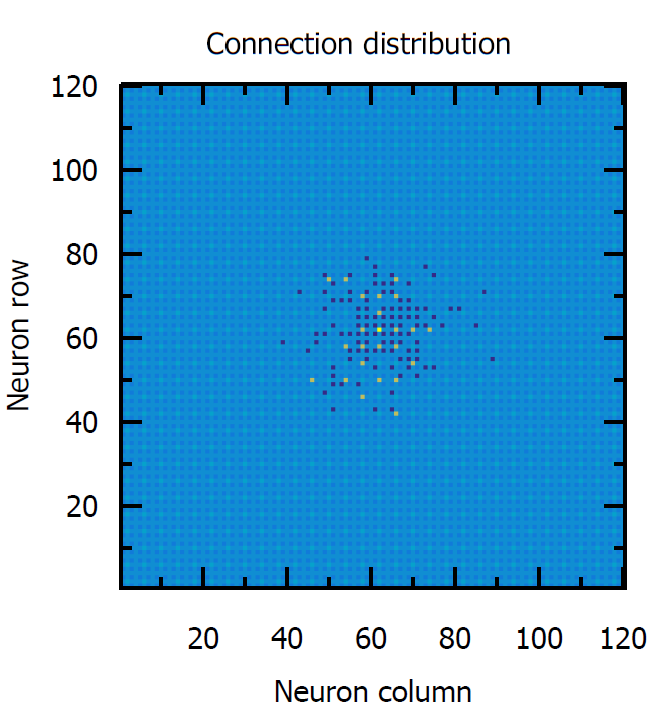
\includegraphics[width = 0.45\textwidth]{connmap.png}
\caption{\textbf{Exemplaric connection map.} Shown are the connections drawn for a specific neuron in the middle of the matrix (light yellow) to excitatory  (deep blue) as well as inhibitory neurons (dark yellow).}
\label{fig:connmap}
\end{figure}
\newline
The input of connected LIF model neurons to a particular neuron is considered using $J_{ji}$ being the efficacy of the individual synapses from neuron \textit{j} to neuron \textit{i} (which are commonly scaled using a coupling strength factor \textit{J}), the connection matrix $m_{ij}$ and an exponential decay of the already existing synaptic input, which is described by the membrane time constant ($decay = exp(-\Delta t/\tau _{synapse}$). The renewing synaptic inputs are then added to the current value for the individual neuron \textit{i} to reflect its total current for a given time step $t+\Delta t$ as is given in Equation \ref{eq:lifgenfinal}: \\
\begin{eqnarray}
\label{eq:lifgenfinal}
I_{internal}(t+ \Delta t) &=& I_{interal,i}(t)  \\ 
& &*exp(\frac{- \Delta t}{\tau _{synapse}}) + \nonumber \\
& & \sum_{j=^1}^{N} w_{ij} \sum_{n_{j}=1}^{N_{k}} \frac{J*J_{ij}}{\tau _{synapse}} \nonumber
\end{eqnarray}

\newpage
\section{Results}
The results are shown separately for excitatory (Chapter \ref{sec:resultex}) and inhibitory neurons (Chapter \ref{sec:resultin}).\newline
If applicable, differences between randomly and Gaussian connected Leaky Integrate-and-Fire neuron models (LIF) are emphasized for single plots as well as generally compared at the end (Chapter \ref{sec:resultgeneral}) over a variety of parameters. \\
Individual plots are not normalized because of the partially very high differences between most plots which would render the comparisons under normalization difficult to trace.
\subsection{Excitatory neurons}
For the following first two analysis, the amplitude and $\sigma$ value for the Gaussian connectivity pattern has been set to 0.41 and 4.00, respectively. The amount of connections drawn for each individual LIF are similar between Gaussian and the random connection pattern.
\label{sec:resultex}
\subsubsection{Coupling strengths}
\begin{figure*} [htp]
\centering
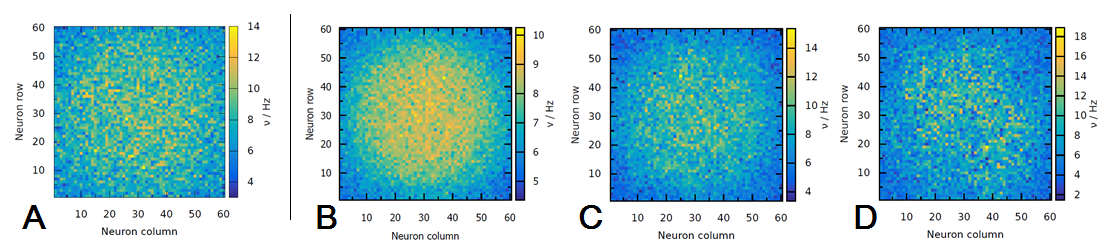
\includegraphics[width = 1.0\textwidth]{ex60_J.png}
\caption{\textbf{Excitatory neurons with differing coupling strengths.} Compared are randomly (A) and Gaussian connected neurons (B-D) with varying coupling strengths of J = 0.2 (B), 1.0 (C) and 2.0 (D). Each LIF incorporates 60'000 channels. Connection probability for random connections was set to $1 \%$ (A), coupling strength is set to 1.0.}
\label{fig:ex60j}
\end{figure*}
First, the general reaction of the network to the stimulus is compared under the two different connectivity patterns. \newline 
By looking at the plots in Figure \ref{fig:ex60j}, one can clearly recognize the applied stimulus as being reflected by the firing rates of the excitatory neurons. This is not only true for the Gaussian connectivity pattern (B-D) but as also for the randomly connected neurons (A). By comparing the plots created under the same coupling strength of J = 1.0 (A and C), the Gaussian connectivity allows slightly higher peaks than the random connectivity pattern with the former having its maximum at a value of about 15 v/Hz and the latter at 14 v/Hz. However, the shape of the stimulus is more specific under Gaussian connectivity with well-defined corners of low activity than for the random pattern.\newline
This can be seen more clearly for lower coupling strengths as in B whereas with a higher factor the resemblance to the original stimulus is less defined with a more wide-spread excitation. The firing rates seem to increase in a rather steady way in response to a change of the synaptic efficacy (from 10 to 15 to about 18 v/Hz) with an drop of the lowest rates from 4 to 2 v/Hz.
\subsubsection{Sensitivity}
\begin{figure*} [htb]
\centering
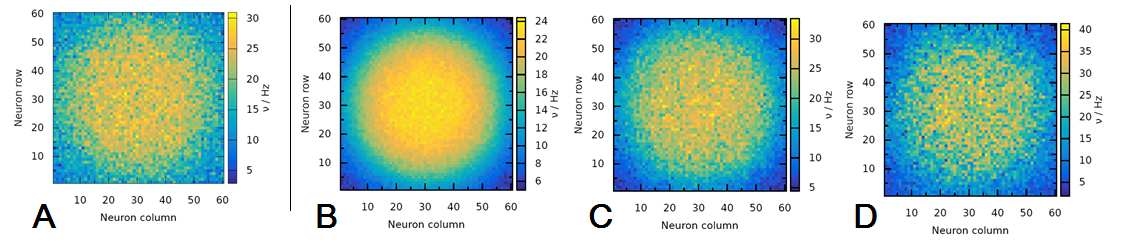
\includegraphics[width = 1.0\textwidth]{ex300_J.png}
\caption{\textbf{Excitatory neurons with differing coupling strengths.} Compared are randomly (A) and Gaussian connected neurons (B-D) with varying coupling strengths of J = 0.2 (B), 1.0 (C) and 2.0 (D). Each LIF incorporates 300'000 channels. Connection probability for random connections was set to $1 \%$ (A), coupling strength is set to 1.0.}
\label{fig:ex300j}
\end{figure*}
Following, we wanted to investigate whether this effect holds for high excitation rates as well. \newline
When the amount of channels a single neuron incorporates is increased from 60'000 to 300'000, the same behavior as described above is still present but yet strengthened (Figure \ref{fig:ex300j}). For the same coupling strength, random and Gaussian connection profiles only differ slightly in their firing rate peaks (A and C) with the latter showing a rather good representation of the stimulus. This is even more visible for lower coupling strengths (B) being nearly a direct copy without much spread and variation of the originally applied stimulus (see Chapter \ref{sec:stimulus}). This, however, is lost partially by increasing the coupling strength (D) which simultaneously increases the highest possible peaks of firing rates. Here, the well-defined shape of the stimulus is spread over a greater area of the network. The lowest firing rates are rather identical for all of those plots with the peaks in a range from 5 to 6 v/Hz (A to D).
\subsubsection{Connectivity degree}
After analyzing the effect a varying amount of light-sensitive channels within the neurons, one may ask what influence the amount and range of possible connections to be drawn might have. For this reason, the amplitude and $\sigma$ of the Gaussian connectivity pattern now has been increased to cover the 10-fold amount of connections with values of 0.60 and 12.00, respectively. \newline
\begin{figure*} [htb]
\centering
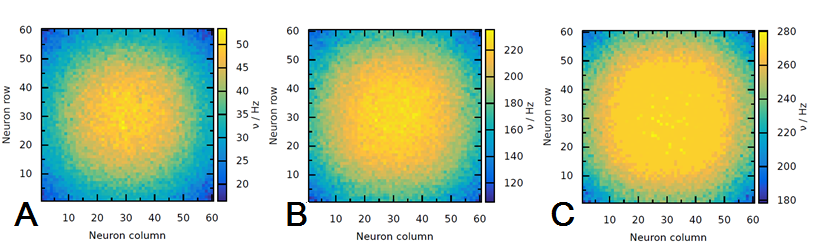
\includegraphics[width = 0.9\textwidth]{ex60_10fold.png}
\caption{\textbf{Excitatory neurons under differing coupling strengths.} Shown are Gaussian connected neurons (A-C) with varying coupling strengths of J = 0.2 (A), 1.0 (B) and 2.0 (C) and a 10-fold amount of connections. Each LIF incorporates 60'000 channels.}
\label{fig:ex6010f}
\end{figure*}
\newline
As it can be seen in Figure \ref{fig:ex6010f}, the shape of the applied stimulus is captured by the neural network only under low coupling strengths. For higher factors, the plots show a high spread of excitation by still holding on to the observed trend for all plots so far with the corners showing low firing rates and the center accordingly high firing rates. \newline
\newline
Additionally, the values for the firing rates increase to a very strong amount between the individual plots by raising the coupling strength. The peak values are quadrupled first (A to B, 55 to 240 v/Hz, coupling strength raise from 0.2 to 1.0) and then reach 280 v/Hz for high couplings strengths by adding a smaller increase. The lowest firing rates found for each plot are increased in the same way with a rapid gain between A and B (about 10 to 110 v/Hz) followed by a less pronounced increased from B to C (110 to 180 v/Hz). 
\subsection{Inhibiitory neurons}
In the next chapter, inhibitory neurons are now of special interest because they do not directly get input from an external source, but only already processed input from the excitatory neurons and they regulate the recurrent excitation. For this reason, they are separately analyzed in the following sections. \newline
For the connections of inhibitory neurons, an amplitude and $\sigma$ of 1.00 and 2.60 has been used for the first analysis to cover the normal amount of connections. For the second analysis, the $\sigma$ value has been raised to 4.00 with the amplitude staying the same to reach a 10-fold amount of connections.
\label{sec:resultin}
\subsubsection{Coupling strength and sensitivity}
\begin{figure*} [htb]
\centering
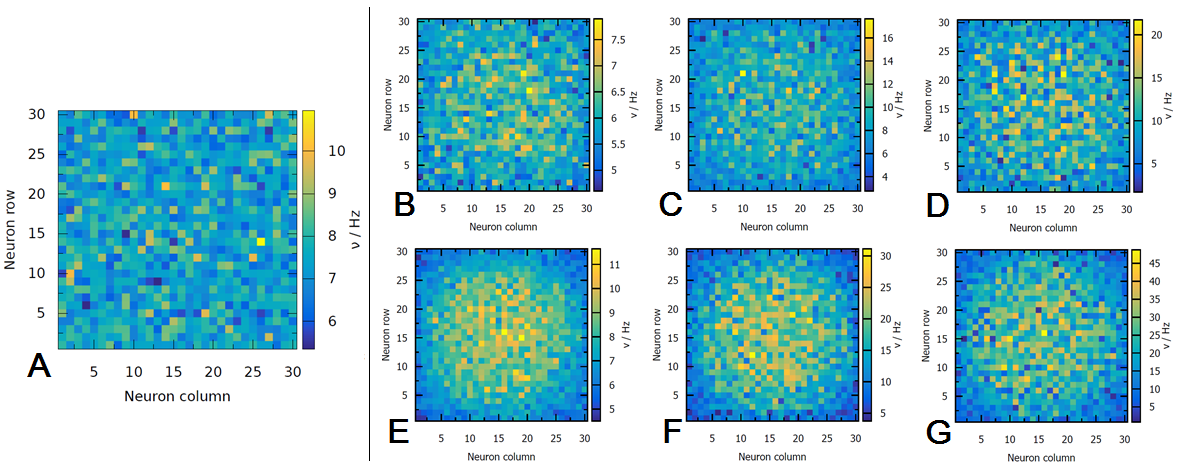
\includegraphics[width = 0.9\textwidth]{in_60300.png}
\caption{\textbf{Inhibitory neurons with differing general coupling strengths and channels within the excitatory population.} Shown are Gaussian connected neurons (B-G) with varying coupling strengths of J = 0.2 (B and E), 1.0 (C and F) and 2.0 (D and G) and different amounts of light-sensitive channels within the excitatory neuron population (60'000 for B-D and 300'000 for E-G). Those are compared to the inhibitory population's reaction using a coupling strength of 1.00 and 60'000 channels within the excitatory population (A).}
\label{fig:in60300}
\end{figure*}
The most striking aspect between the individual plots of Figure \ref{fig:in60300} is the highly unordered structure of the random connectivity pattern compared with those having a Gaussian connectivity pattern applied. This difference is already visible for low coupling strengths (B) and a smaller excitation of the excitatory population (as being caused by 60'000 channels, B to D) but becomes very strong for high excitatory firing rates due to 300'000 light-sensitive channels (E to G). The visually strongest resemblance to the applied stimulus can there be seen at high coupling strengths (E). \newline
Overall, the general behavior which has been found for the excitatory population is reflected by the inhibitory population as well, showing an peak of firing rates (from around 8 over 18 to 22 v/Hz for 60'000 channels and 12 over 30 to 48 v/Hz for 300'000 channels, resp.) with the lowest values staying within the same range (between 3 and 5 v/Hz).\newline
Additionally, it is worth indicating that the highest firing rates are found for the random connectivity pattern is much lower than for the corresponding plot using Gaussian distributed connections (C) as well where there has only been a slight difference for excitatory populations. 
\subsubsection{Connectivity degree}
\begin{figure*} [htb]
\centering
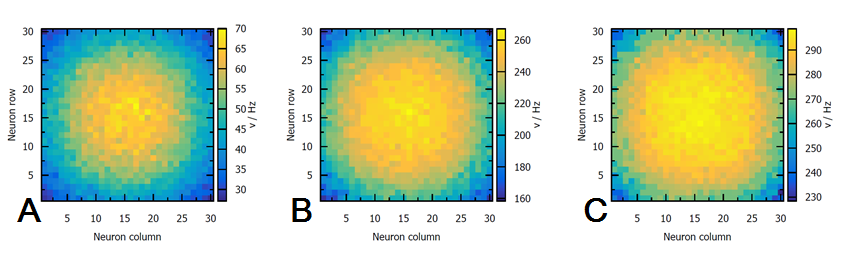
\includegraphics[width = 0.9\textwidth]{in_60_10fold.png}
\caption{\textbf{Inhibitory neurons under differing general coupling strengths} Shown are Gaussian connected neurons (A-C) with varying coupling strengths of J = 0.2 (A), 1.0 (B) and 2.0 (C) and a 10-fold amount of connections as achieved by using an amplitude of 1.00 and $\sigma$ of 4.00 for the connectivity pattern following a Gaussian distribution.}
\label{fig:in6010f}
\end{figure*}
The plots in Figure \ref{fig:in6010f} are rather similar to those obtained for the excitatory population (Figure \ref{fig:ex6010f}). The Corners tend to remain at relative lower firing rates with the peak area spreading over the network by increasing the coupling strength between synapses. Again, as seen for the excitatory neurons, there is a rapid increase in firing rates between lower and medium coupling strengths (A to B, 70 to 270 v/Hz) with only a small addition for a higher factor (C, 300 v/Hz). 
\subsection{Random vs Gaussian pattern}
\begin{figure*} [htp]
\centering
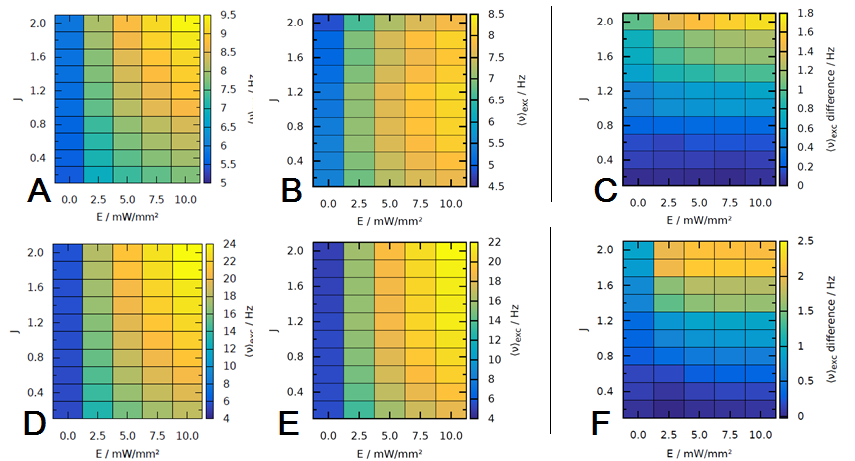
\includegraphics[width = 0.9\textwidth]{ex_tileplot.png}
\caption{\textbf{Tile plots of excitatory populations} Shown are tile plot for a varying coupling strength, stimulus strength and the resulting firing rates of the excitatory population with 60'000 (A to C) or 300'000 channels (D to F) distinguished into plots for randomly drawn connections (A and D) as well as Gaussian connectivity profiles (B and E) as well as the difference plots (C and F). Networks consist of 4500 neurons (3600 of which are excitatory and 900 inhibitory).}
\label{fig:tileplotex}
\end{figure*}
As it can be seen in Figure \ref{fig:tileplotex}, the total differences between randomly and Gaussian connected populations are only small with the highest differences being found at strong stimuli and higher coupling strengths (A and B, D and E). Beside of this, the networks react rather similar to the input. The difference plots (C and F) show that the overall firing rate is always higher for random connection patterns than for a specific pattern being applied following the trend that an increase in coupling strength or stimulus strength increases the difference between the different connectivity patterns along with the individual firing rates. \newline
This is not only true for 60'000 channels incorporated by a single neuron (A to C), but also for 300'000 as well (D to F).\newline
\begin{figure} [htp]
\centering
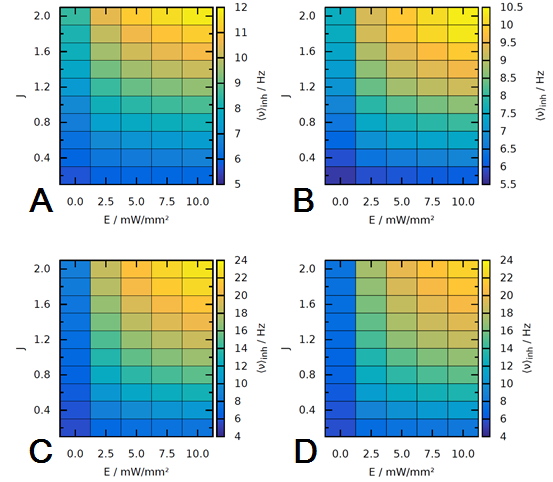
\includegraphics[width = 0.5\textwidth]{in_tileplot.png}
\caption{\textbf{Tile plots of inhibitory populations} Shown are tile plot for a varying coupling strength, stimulus strength and the resulting firing rates of the inhibitory population with each neuron of the excitatory population incorporating 60'000 (A and B) or 300'000 channels (C and D) distinguished into plots for randomly drawn connections (A and C) as well as Gaussian connectivity profiles (B and D).}
\label{fig:tileplotin}
\end{figure}
\newline
For networks with 60'000 channelrhodopsin-2 channels, the tile plots in Figure \ref{fig:tileplotin} show the same behavior as for the excitatory population with the Gaussian connected network establishing generally lower total firing rates. These rates are smallest for low coupling and stimulus strengths and increase when one of them is risen.\newline
The plots for 300'000 channels show only a very subtle difference between both connectivity patterns but are otherwise extremely similar.
\label{sec:resultgeneral}
\newpage
\section{Discussion}
The main aspect and most significant outcome seen clearly in the results is the different reaction of the inhibitory population to the evoked excitation within the network. While there is no detectable pattern for the randomly connected network, even for a small excitation and all variations of coupling strengths a specific reaction can be seen for the Gaussian connectivity pattern (Figure \ref{fig:in60300}). This becomes especially obvious for high excitation (due to an increased amount of channels, raising from 60'000 to 300'000) and shows how the inhibitory reaction is dependent on the connectivity pattern of both excitatory and inhibitory neurons.  \newline
Of course this depends on the individual connections drawn for a single neuron were here only the assumption of a neuron's tendency to connect to closer neighboring neurons has been implemented without values as derived from real biological systems. But even under this simplified assumption, the behavior could be found being present for all coupling strengths and amounts of excitation and is true as well for very high connectivities as could be seen in Figure \ref{fig:in6010f}) but could not be seen for the random connectivity pattern in despite of the same stimulus being applied to to network.\newline
\newline
The behavior mentioned above on the one hand and the underlying connectivity pattern on the other hand lead to higher peaks of firing rates found for Gaussian connected networks with the mean over the whole network always being smaller than for random connections. This is explainable considering the strong reflection of the actual stimulus which has a small peak area with a high intensity which drops following a Gaussian distribution towards points further away from the center. As a result, this creates large and well-defined areas at the corners with low firing rates leading to a smaller mean of the whole network. It is interesting how this behavior is reflected by the inhibitory population. Especially the very similar firing rates of the inhibitory population (\ref{fig:tileplotin}, C and D) for a high amount of light sensitive channels and corresponding activity within the excitatory population still leading to smaller mean firing rates of the excitatory population are questionable. This could be explained by limitations of the network and dynamics originating in the Gaussian distribution or the result of computational issues. Considering the individual plots of the inhibitory population for a lower excitation of excitatory neurons (with 60'000 channels), neurons feature the same behavior as the excitatory population with higher peak firing rates and a lower mean, following the same reasoning as above. \newline
\newline
The extremely high firing rates for high connectivities seen for the inhibitory and excitatory populations, however, show that there is a critical amount of connections for a specific stimulus and neuron type leading to rather unhealthy, or even pathological, behaviors. Here, the feedforward aspect of the network drives the high firing rate values which are only restricted by the implementation of the neuron models and brought to its limits. By modeling different types of connections, a stronger inhibition and e.g. synaptic normalization mechanisms, this behavior could possibly be altered. The amount of connections used are, however, rather unrealistic by incorporating nearly the whole network and serve only demonstrative purposes. \newline
Nevertheless, the spread of the peak area which is clearly visible within these plots could be generally observed for higher coupling strengths as well as for both populations even when having a more realistic number of connections. This leads to the assumption that a specific response to a stimulus might be hard to achieve without specific connections drawn in relation to the expected stimulus. In order to keep the characteristics of such a special activation, the connections have to be created in a similar special way to avoid over-excitation and pathological behavior.\newline
Therefore, it could not only be shown that the strength and shape of the response within such a network is determined by the underlying connectivity, but also that the amount of connections needed for a specific response (e.g. a target firing rate) depends on the connections of the neurons as well.
\section{Outlook}
Because the analysis performed in this module are only of a qualitative aspect, the studies could be extended to more biologically realistic values for the Gaussian connectivity distributions to model different target areas and ranges of connectivity as found for various neurons. \newline
Alongside, more detailed distributions could be implemented, having for example random connections for excitatory neurons and Gaussian distributed connections for inhibitory neurons or individual target areas for single neurons. This includes different kinds of inhibition as well as feed-forward, feedback and lateral inhibition.
%\begin{samepage} 
%\label{sec:appendix}
\begin{thebibliography}{999}
\bibitem [Abbott (1999)] {abbott} Abbott, F. (1999). Lapique's introduction of the integrate-and-fire model neuron (1907), Brain Research Bulletin 50 (5/6): 303–304. doi:10.1016/S0361-9230(99)00161-6. PMID 10643408.
\bibitem [Bassett and Bullmore (2006)] {Bassett} Bassett, D., Bullmore, E. (2006) Small world brain networks. Neuroscientist. 2006 Dec;12(6):512-23. PMID: 17079517; DOI: 10.1177/1073858406293182 
\bibitem [Crook, Kisvarday and Eysel (1997)] {Crook} Crook, J., Kisvarday, Z., Eysel, U. (1997) GABA-induced inactivation of functionally characterized sites in cat striate cortex: effects on orientation tuning and direction selectivity. Vis Neurosci 14:141–158
\bibitem [Deisseroth (2015)] {deisseroth} Deisseroth, K. (2015). Optogenetics: 10 years of microbial opsins in neuroscience. Nature
Neuroscience 18.
\bibitem [Engel, Fries and Singer (2001)] {engel} Engel A.K., Fries P., Singer W. (2001) Dynamic predictions: oscillations and synchrony in top-down processing. Nat. Rev. Neurosci. 2:704-716. 
\bibitem [Gradinaru et al. (2009)] {gradinaru} Gradinaru, V., Mogri, M., Thompson, K. R., Henderson, J. M., and Deisseroth, K.
April 2009. Optical Deconstruction of Parkinsonian Neural Circuitry. Science 324.
\bibitem [Haubensak et al. (2010)] {Haubensak} Haubensak, W.; Kunwar, P. S.; Cai, H.; Ciocchi, S.; Wall, N. R.; Ponnusamy, R.; Biag, J.; Dong, H. W.; Deisseroth, K.; Callaway, E. M.; Fanselow, M. S.; Lüthi, A.; Anderson, D. J. (2010). Genetic dissection of an amygdala microcircuit that gates conditioned fear. Nature 468 (7321): 270–276. doi:10.1038/nature09553. PMC 3597095. PMID 21068836.
\bibitem [Hermandez et al. (2014)] {hermandez} Hernandez, V.; et al. (2014). Optogenetic stimulation of the auditory pathway. J Clin Invest 124 (3): 1114–1129. doi:10.1172/JCI69050. PMC 3934189. PMID 24509078.
\bibitem [Hodgkin and Huxley (1952)] {Hodgkin} Hodgkin, A. L., Huxley, A. F. (1952). A quantitative description of membrane current and its application to conduction and excitation in nerve. The Journal of Physiology 117 (4): 500–544. doi:10.1113/jphysiol.1952.sp004764. PMC 1392413. PMID 12991237.
\bibitem [Jannik Luboeinski (2016)] {jannik} Luboeinski, J. (2016). Modeling of a neural network with integrated light-sensitive channels. Master's thesis.
\bibitem [Nagel et al (2003)] {nagel} Nagel, G., Szellas, T., Huhn, W., Kateriya, S., Adeishvili, N., Berthold, P., Ollig, D., Hegemann, P., and Bamberg, E. (2003). Channelrhodopsin-2, a directly light-gated cation-selective membrane channel. Proc. Natl. Acad. Sci. USA 100.
\bibitem [Nossenson and Messer (2010)] {Nossenson} Nossenson, N., Messer, H. (2010). Modeling neuron firing pattern using a two state Markov chain. Sensor Array and Multichannel Signal Processing Workshop (SAM), 2010 IEEE. Piscataway, NJ: IEEE 117 (4): 500–544.
\bibitem [Salinas and Sejnowski (2001)] {salinas} Salinas E., Sejnowski T.J. (2001) Correlated neuronal activity and the flow of neural information. Nat. Rev. Neurosci. 22:539-550.
\bibitem [Siebert (1965)] {siebert} Siebert, W. (1965). Some implications of the stochastic behavior of primary auditory neurons. Kybernetik 2 (5): 206–215. doi:10.1007/BF00306416. ISSN 0023-5946.
\bibitem [Sporns et al. (2004)] {sporns} Sporns, O., Chialvo D., Kaiser M., Hilgetag C. (2004). Organization, development and function of complex brain networks. Trends Cogn Sci. 8 (9): 418–425. PMID 15350243.
\bibitem [Zemelman and Miesenböck (2002)] {zemelmann} Zemelman, B. V., Lee, G. A.; Ng, M., Miesenböck, G. (2002). Selective photostimulation of genetically chARGed neurons. Neuron 33 (1): 15–22. doi:10.1016/S0896-6273(01)00574-8. PMID 11779476.
\end{thebibliography}
\end{document}